%-------------------------------------------------------------------------------
%                            BAB II
%               TINJAUAN PUSTAKA DAN DASAR TEORI
%-------------------------------------------------------------------------------
\fancyhf{} 
\fancyfoot[C]{\thepage}
\chapter{TINJAUAN KEPUSTAKAAN}               

\section{\uppercase{HIDROPONIK}}
Istilah hidroponik (Inggris: \textit{hydroponic}) berasal dari kata Yunani yaitu \textit{hydro} yang berarti air dan \textit{ponos} yang berarti daya. Hidroponik juga dikenal sebagai \textit{soilless culture} atau budi daya tanaman tanpa tanah. Secara umum, hidroponik merupakan budi daya menanam tanpa tanah, akan tetapi dengan memanfaatkan air dan lebih menekankan pada pemenuhan kebutuhan nutrisi tanaman \citep{alviani2015bertanam}.

\par Hidroponik mempunyai berbagai kelebihan apabila dibandingkan dengan bercocok tanam sistem konvensional, antara lain adalah tidak menuntut lahan yang luas sehingga mungkin diterapkan oleh masyarakat perkotaan dengan ketersediaan lahan kosong yang terbatas, lokasi penanaman bisa di mana saja, pilihan jenis tanaman yang bisa ditanam sangat beragam, tingkat pertumbuhan yang lebih cepat sehingga lebih cepat dipanen, dan teknis perawatannya relatif tidak sulit sehingga bisa dipraktikkan oleh hampir semua orang \citep{iqbal2016simpel}.

\section{\uppercase{PEMASARAN DIGITAL}}
Menurut \citep{tarigan2013creative} “Pemasaran Digital adalah kegiatan pemasaran termasuk \textit{branding} yang menggunakan berbagai media berbasis web seperti blog, \textit{website, e-mail, adwords}, ataupun jejaring sosial. Tentu saja pemasaran digital bukan hanya berbicara tentang pemasaran internet.”

Pemasaran digital adalah salah satu media pemasaran yang saat ini sedang banyak diminati oleh masyarakat untuk mendukung berbagai kegiatan yang dilakukan. Masyarakat sedikit demi sedikit mulai meninggalkan model pemasaran konvensional/tradisional beralih ke pemasaran modern yaitu pemasaran digital. Dengan pemasaran digital komunikasi dan transaksi dapat dilakukan setiap waktu/\textit{real time} dan bisa mengglobal atau mendunia. Dengan jumlah pengguna media sosial berbasis \textit{chat} ini yang banyak dan semakin hari semakin bertambah membuka peluang bagi UKM untuk mengembangkan pasarnya dalam genggaman \textit{smartphone} \citep{pradiani2017pengaruh}.

\section{\uppercase{E-COMMERCE}}
Menurut \citep{yuhefizar2013}, “\textit{e-commerce} adalah singkatan dari \textit{electronic commerce}, yaitu sebuah layanan berbasis elektronik (internet) untuk bertransaksi/berdagang secara \textit{online}.” Sedangkan menurut \citep{saputra2013}, “\textit{e-commerce} adalah segala aktivitas transaksi produk ataupun jasa antara penjual dan pembeli dengan memanfaatkan kecanggihan elektronik, sehingga proses transaksi dapat dilakukan meskipun antara penjual dan pembeli tidak secara langsung bertatap muka.”

\fancyhf{} 
\fancyfoot[R]{\thepage}

Menurut \citep{pradana2015klasifikasi} terdapat enam model bisnis \textit{e-commerce} yang berkembang di Indonesia, antara lain:

\begin{enumerate}
	\item \textit{Classifieds/listing}/iklan baris, adalah model bisnis \textit{e-commerce} paling sederhana dan cocok digunakan di negara-negara berkembang. Dua kriteria yang biasa diusung oleh model bisnis ini adalah \textit{website} yang bersangkutan tidak memfasilitasi kegiatan transaksi \textit{online} penjual individual, dapat menjual barang kapan saja, di mana saja dan dilakukan secara gratis. Contoh situs iklan baris yang terkenal di Indonesia ialah OLX.
	\item \textit{Marketplace} C2C (\textit{Customer to Customer}), ini adalah model bisnis di mana \textit{website} yang bersangkutan tidak hanya membantu mempromosikan barang dagangan saja, tapi juga memfasilitasi setiap transaksi. Indikator utama bagi sebuah \textit{website} \textit{marketplace} adalah harus memfasilitasi transaksi \textit{online} dan harus dapat digunakan oleh penjual individual.
	Contoh \textit{marketplace} di Indonesia yang memperbolehkan pihak penjual untuk langsung menjual produknya di \textit{website} ialah Tokopedia, Bukalapak, dan Shopee. Namun ada juga situs \textit{marketplace} lainnya yang mengharuskan penjual menyelesaikan proses verifikasi terlebih dahulu seperti Blanja dan Elevenia.
	\item \textit{Shopping mall}, ialah model bisnis yang memiliki kesamaan dengan \textit{marketplace}, tapi penjual yang bisa berjualan di situs ini hanya penjual yang menjual produk dengan \textit{brand} ternama atau menjual produk-produk original, karena proses verifikasi yang ketat. Contoh situs \textit{online shopping mall} yang beroperasi di Indonesia ialah Blibli.
	\item Toko \textit{online} B2C (\textit{Business to Consumer}), model bisnis ini cukup sederhana, yakni sebuah toko \textit{online} dengan alamat \textit{website} (\textit{domain}) sendiri, di mana pihak penjual memiliki stok produk dan menjualnya secara \textit{online} kepada pembeli.
	Beberapa contoh toko \textit{online} terkenal di Indonesia ialah Bhinneka, Tiket.com, dan BerryBenka.
	\item Toko \textit{online} di media sosial, banyak sekali penjual di Indonesia yang memanfaatkan situs media sosial seperti Facebook dan Instagram untuk mempromosikan barang dagangan mereka. Bisnis model seperti ini cocok untuk penjual yang ingin menjual produk maupun jasanya, namun belum memiliki toko fisik. Tetapi, di era modern sekarang ini, bahkan hampir semua penjual yang sudah memiliki toko fisik tetap menggunakan media sosial sebagai sarana menjual dan mempromosikan barangnya, karena prosesnya yang mudah dan dapat dijalankan secara gratis.
	\item Jenis-jenis \textit{website crowdsourcing} dan \textit{crowdfounding}, \textit{website} ini dipakai sebagai platform untuk mengumpulkan orang-orang dengan \textit{skill} yang sama atau untuk penggalangan dana secara \textit{online}.
	Beberapa contoh webnya seperti kitabisa.com, wujudkan.com dan sebagainya.
\end{enumerate}

\section{\uppercase{WEBSITE}}
\textit{World Wide Web} atau yang lebih dikenal dengan istilah web (\textit{website}) adalah sistem pengaksesan informasi dalam internet. Web disusun dari halaman–halaman yang menggunakan teknologi web dan saling berkaitan satu sama lain. Sedangkan pengertian lain menyebutkan bahwa \textit{website} adalah rangkaian atau sejumlah halaman web di internet yang memiliki topik saling berkaitan untuk mempresentasikan suatu informasi \citep{ginanjar2014rahasia}.

\par \textit{Website online} harus memiliki domain. Sebuah domain atau alamat web dibuat dengan menggunakan “\textit{Domain Name System}” yang merupakan metode yang dipakai untuk mengorganisir seluruh nama–nama komputer yang ada di internet. Contoh domain adalah .com (komersil atau bisnis), .gov (pemerintahan), .mil (militer), .net (institusi yang berbeda), dan .ac (institusi pendidikan). Untuk top domain .id (Negara Indonesia), .ca (Negara Canada), .us (Negara Amerika) dan sebagainya yang berarti kepemilikan web negara \citep{dhika2015perancangan}.

\section{\uppercase{ENTITY RELATIONSHIP DIAGRAM (ERD)}}
Menurut \citep{priyadi2014} menyatakan bahwa : Pemodelan basis data dengan menggunakan diagram relasi antara entitas, dapat dilakukan dengan menggunakan suatu pemodelan basis data yang bernama Diagram \textit{Entity Relationship} yang disingkat Diagram E-R. ERD juga merupakan gambaran yang menghubungkan antara objek satu dengan objek yang lain dalam dunia nyata. Bisa dikatakan bahwa bahan yang akan digunakan untuk membuat ERD adalah dari objek di dunia nyata. Secara umum ERD terdiri dari 4 komponen, yakni :

\begin{enumerate}
	\item Entitas
	\par Entitas merupakan notasi untuk mewakili suatu objek dengan karakteristik sama, yang dilengkapi oleh atribut, sehingga pada suatu lingkungan nyata objek akan berbeda dengan objek lainnya.
	\pagebreak
	\item Relasi
	\par Relasi merupakan notasi yang digunakan untuk menghubungkan beberapa entitas berdasarkan fakta pada suatu lingkungan.
	\item Atribut
	\par Atribut merupakan notasi yang menjelaskan karakteristik suatu entitas dan juga relasinya. Atribut dapat sebagai \textit{key} yang bersifat unik, yaitu \textit{primary key} atau \textit{foreign key}. Selain itu, atribut juga dapat sebagai atribut deskriptif saja, yaitu sebagai pelengkap deskripsi suatu entitas dan relasi.	
	\item Garis Penghubung
	\par Garis penghubung merupakan notasi untuk merangkai keterkaitan antara notasi-notasi yang digunakan dalam Diagram E-R , yaitu entitas, Relasi , dan atribut.
\end{enumerate}

\section{\uppercase{UNIFIED MODELING LANGUAGE (UML)}}
Menurut \citep{nugraha2016perancangan} UML yang biasa disebut (\textit{Unified Modeling Language}) adalah sebuah bahasa pemodelan untuk sistem atau \textit{software} yang berkonsep berorientasi objek. UML seharusnya digunakan untuk perancangan model sebuah sistem yang lengkap sedemikian rupa sehingga sangat mudah untuk dipelajari dan dipahami. Beberapa jenis UML yang dipakai dalam pengembangan aplikasi yaitu model \textit{Use Case Diagram, Class Diagram} dan \textit{Activity Diagram}. Berikut adalah penjelasannya:

\begin{enumerate}[a.]
	\item \textit{Use Case Diagram}
	\par \textit{Use Case Diagram} menggambarkan fungsionalitas yang diharapkan dari sebuah sistem. \textit{Use case} merupakan sebuah pekerjaan tertentu, misalnya \textit{login}, men-\textit{create} sebuah bukti transaksi, dan sebagainya. Sebuah aktor adalah sebuah entitas manusia atau mesin yang berinteraksi dengan sistem untuk melakukan pekerjaan-pekerjaan tertentu.
	\item \textit{Class Diagram}
	\par \textit{Class Diagram} menggambarkan struktur dan deskripsi \textit{class, package} dan objek beserta hubungan satu sama lain seperti \textit{containment}, pewarisan, asosiasi, dan lain-lain.
	\item \textit{Activity Diagram}
	\par \textit{Activity Diagram} menggambarkan berbagai alur aktivitas dalam sistem yang sedang dirancang, bagaimana masing-masing alur berawal, \textit{decision} yang mungkin terjadi, dan bagaimana mereka berakhir. \textit{Activity diagram} juga dapat menggambarkan proses paralel yang mungkin terjadi pada beberapa eksekusi.
\end{enumerate}

\section{\uppercase{LARAVEL LIVEWIRE}}
Laravel merupakan sebuah kerangka kerja yang dikembangkan oleh Taylor Otwell di MIT dengan basis bahasa pemrograman PHP (\textit{Hypertext Preprocessor}) yang bersifat \textit{Open Source} di mana Laravel ini menggunakan kerangka arsitektur MVC (\textit{Model-View-Controller}) di mana komponen pada Laravel sangat mudah untuk dipahami seperti fitur \textit{authentication}, \textit{session manager}, \textit{routing}, dan \textit{caching}, kemudian fitur Unit Testing \textit{Support} yang telah terintegrasi untuk seorang pengembang laman web agar lebih mudah dalam mengembangkan aplikasi yang kompleks \citep{sebastian2021perancanagan}.

\par Livewire adalah kerangka kerja \textit{full-stack} untuk Laravel yang membuat membangun antarmuka dinamis menjadi sederhana, tanpa meninggalkan kenyamanan Laravel \citep{livewire2021}. Cara kerja dari Livewire adalah sebagai berikut:

\begin{itemize}
	\item Livewire merender \textit{output} komponen awal dengan halaman (termasuk seperti \textit{Blade}), dengan cara ini SEO \textit{friendly}.
	\item Ketika interaksi terjadi, Livewire membuat permintaan AJAX ke server dengan data yang diperbarui.
	\item Server merender ulang komponen dan merespons dengan HTML baru.
	\item Livewire kemudian dengan cerdas mengubah DOM sesuai dengan hal-hal yang berubah.
\end{itemize}

% \begin{figure}[H]
% \centering
% {
\includegraphics [width = 10.5cm, height= 6cm]{gambar/laravel-livewire}}
% \caption{Laravel Livewire \citep{krishaweb2021}}
% \label{laravel_livewire}
% \end{figure}

\section{\uppercase{MySQL}}
MySQL adalah salah satu program yang dapat digunakan sebagai \textit{database}, dan merupakan salah satu \textit{software} untuk \textit{database} server yang banyak digunakan. MySQL bersifat \textit{open source} dan menggunakan SQL. MySQL bisa dijalankan di berbagai platform misalnya Windows, Linux, dan lain sebagainya. MySQL memiliki kelebihan, antara lain: \citep{orlando2017aplikasi}

\begin{enumerate}
	\item Dapat digunakan oleh beberapa \textit{user} dalam waktu yang bersamaan tanpa mengalami masalah.	
	\item Memiliki kecepatan yang bagus dalam menangani \textit{query} sederhana.
	\item Memiliki operator dan fungsi secara penuh dan mendukung perintah \textit{select} dan \textit{where} dalam perintah \textit{query}.
	\item Memiliki keamanan yang bagus karena beberapa lapisan sekuritas seperti level \textit{subnetmask}, nama \textit{host}, dan izin akses \textit{user} dengan sistem perizinan yang mendetail serta sandi terenkripsi.
	\item Mampu menangani basis data dalam skala besar, dengan jumlah rekaman lebih dari 50 juta dan 60 ribu tabel serta kurang lebih 5 milyar baris. Selain itu batas indeks yang dapat ditampung mencapai 32 indeks pada tiap tabelnya
\end{enumerate}

\section{\uppercase{WEB SERVICE}}
\textit{Web service} adalah salah satu bentuk sistem perangkat lunak yang didesain untuk mendukung interaksi mesin ke mesin melalui jaringan. \textit{Web service} memiliki \textit{interface} yang dideskripsikan dalam format yang dapat dibaca oleh mesin \citep{prabowo2016teknologi}. Kasman mengemukakan, “\textit{Web Service} adalah aplikasi yang dibuat agar dapat dipanggil dan diakses oleh aplikasi lain melalui internet dengan menggunakan format pertukaran data sebagai format pengiriman pesan” \citep{kasman2015}.

\textit{Web service} digunakan sebagai salah satu fasilitas yang disediakan oleh suatu web untuk menyediakan layanan dalam bentuk informasi kepada sistem lain, sehingga sistem lain dapat berinteraksi dengan sistem tersebut melalui layanan \textit{service} yang disediakan oleh suatu sistem yang menyediakan \textit{web service}.” Pada penelitian ini akan digunakan \textit{web services} dengan layanan protokol REST untuk membantu aplikasi penjualan tanaman hidroponik berbasis Android berinteraksi dengan \textit{database} yang terdapat di web server.

\section{\uppercase{REST}}
REST (\textit{Representational State Transfer}) merupakan standar arsitektur komunikasi berbasis web yang sering diterapkan dalam pengembangan layanan berbasis web atau sistem terdistribusi. RESTful \textit{web service} atau juga dikenal dengan nama RESTful Web API merupakan sebuah \textit{web service} yang di implementasikan dengan menggunakan HTTP dengan menggunakan prinsip-prinsip REST. Istilah REST diperkenalkan oleh Roy Fielding pada tahun 2000. Arsitektur gaya REST adalah arsitektur klien server di mana klien mengirim permintaan ke server, server kemudian memproses permintaan dan mengembalikan tanggapan. Umumnya menggunakan HTTP (\textit{Hypertext Transfer Protocol}) sebagai protokol untuk komunikasi data \citep{saputra2018}.

\par Berikut metode HTTP yang umum digunakan dalam arsitektur berbasis REST:
\begin{enumerate}
	\item GET, menyediakan hanya akses baca pada \textit{resource}.
	\item PUT, digunakan untuk menciptakan \textit{resource} baru.
	\item DELETE, digunakan untuk menghapus \textit{resource}.
	\item POST, digunakan untuk memperbarui \textit{resource} yang ada atau membuat \textit{resource} baru.
	\item OPTIONS, digunakan untuk mendapatkan operasi yang di \textit{support} pada \textit{resource}.
\end{enumerate}

\section{\uppercase{VIRTUAL PRIVATE SERVER (VPS)}}
\textit{Virtual Private Server} (VPS) adalah \textit{virtual machine} yang dijual sebagai layanan oleh \textit{hosting provider}, dalam VPS \textit{user} bisa mengakses dan mengelola seluruh aspek \textit{software} dari server termasuk akses administrator di sistem oprasi server sampai aplikasi yang akan di implementasikan di server tersebut. VPS dapat dibagi menjadi beberapa VM \textit{(Virtual Machines)}, di mana di setiap VM adalah berupa \textit{“Virtual server”} yang dapat di \textit{install} sistem operasi tersendiri. VPS terasa seperti sebuah \textit{Dedicated Server}. Dibanding dengan \textit{shared hosting}, menyewa VPS akan mendapatkan \textit{resource} yang lebih baik sehingga tidak terganggu jika ada problem pada \textit{website} yang dikelola. Selain itu VPS mendapatkan \textit{root} akses sehingga lebih leluasa dalam melakukan kustomisasi server sesuai kebutuhan \citep{hamida2017analisis}.

\section{\uppercase{SCRUM}}
Scrum dikembangkan oleh Jeff Sutherland pada tahun 1993 untuk menciptakan metode pengembangan yang mengikuti prinsip-prinsip metode \textit{Agile} \citep{fernando2018rancang}. Scrum merupakan satu metode \textit{Agile} paling popular. Metode ini merupakan metode adaptif, cepat, fleksibel, dan efektif serta dapat memberikan hasil yang signifikan dengan cepat \citep{hadinata2017implementasi}.

\par Scrum adalah sebuah kerangka kerja untuk pengembangan tambahan yang menggunakan satu atau lebih tim \textit{cross} fungsional. Scrum menggunakan iterasi tetap yang disebut \textit{sprint}, yang berlangsung selama satu hingga empat minggu. Tim Scrum berusaha untuk menghasilkan peningkatan yang telah diuji di setiap iterasi. Alur metode Scrum dapat dilihat pada gambar \ref{scrum}.

\begin{figure}[H]
\centering
{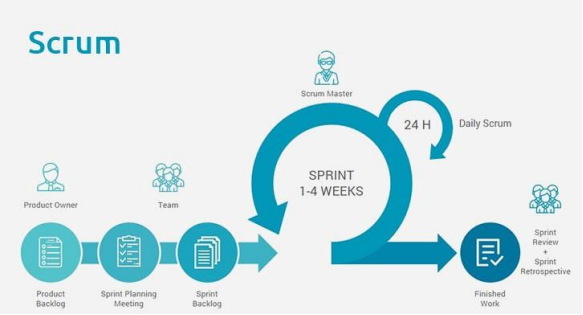
\includegraphics [width = 12.5cm, height= 7cm]{gambar/scrum}}
\caption{Metode Scrum \citep{wahyudi2018analisis}}
\label{scrum}
\end{figure}	

\par Scrum menurut \citep{wahyudi2018analisis} adalah salah satu metode pengembangan aplikasi dengan pengimplementasian proses \textit{Agile Development}. Scrum mempunyai perbedaan yang signifikan dikarenakan produk yang dihasilkan akan menyesuaikan dengan lingkungan seiring waktu proses pengembangan berlalu.

\section{\uppercase{BLACK BOX TESTING}}
\textit{Black Box Testing} berfokus pada pengujian dari masing-masing spesifikasi fungsional perangkat lunak. Seorang tester dapat mendefinisikan kumpulan kondisi \textit{input} dan melakukan pengetesan pada fungsionalitas perangkat lunak \citep{mustaqbal2015pengujian}. Metode \textit{Black Box testing} terdiri atas beberapa metode, antara lain \textit{Equivalence Partitioning}, \textit{Boundary Value Analysis}, \textit{State Transition Testing}, dan \textit{Decision Table Testing}.

\par \textit{Black Box Testing} merupakan metode pengujian perangkat lunak yang digunakan untuk menguji sebuah perangkat lunak tanpa 
mengetahui struktur internal kode atau program. Dalam pengujiannya, penguji menyadari apa yang harus dilakukan oleh program, tapi tidak memiliki pengetahuan tentang bagaimana melakukannya. Kelebihan \textit{black box testing} yaitu :

\begin{enumerate}
	\item Efisien untuk segmen kode besar.
	\item Akses kode tidak diperlukan.
	\item Pemisahan antara perspektif pengguna dan pengembang.
\end{enumerate}

\par Selain memiliki kelebihan, \textit{black box testing} juga memiliki kelemahan, yaitu:

\begin{enumerate}
	\item Cakupan terbatas karena hanya sebagian kecil dari skenario pengujian yang dilakukan. 
	\item Pengujian tidak efisien karena keberuntungan tester dari pengetahuan tentang perangkat lunak internal.
\end{enumerate}

\section{\uppercase{USABILITY MATRIC FOR USER EXPERIENCE (UMUX)}}
UMUX lebih luas daripada kuesioner \textit{single ease question}, tetapi lebih pendek dari standar industri, SUS (\textit{System Usability scale}). UMUX menggunakan skala \textit{likert} 7 poin dan 4 item pertanyaan yang digunakan untuk penilaian subjektif dari kegunaan yang dirasakan situs web, aplikasi atau perangkat lunak lainnya. UMUX dirancang untuk memberikan hasil yang serupa dengan yang diperoleh SUS pada 10 item \textit{usability}, dan diatur berdasarkan definisi \textit{usability} ISO 9241-11 \citep{wahyuningrum2021buku}.

\par Penelitian \citep{finstad2010usability} menunjukkan bahwa kedua skala, baik UMUX maupun SUS berkorelasi baik, dapat diandalkan, dan keduanya selaras pada satu faktor \textit{usability} yang mendasarinya. Selain itu, UMUX cukup ringkas untuk berfungsi sebagai modul \textit{usability} dalam metrik pengalaman pengguna yang lebih luas. Item pertanyaan pada kuesioner UMUX dapat dilihat sebagai berikut:

\begin{enumerate}
	\item Sistem ini mampu memenuhi persyaratan saya.
	\item Menggunakan sistem ini merupakan pengalaman yang frustasi.
	\item Sistem ini mudah untuk digunakan.
	\item Saya memerlukan lebih banyak waktu untuk memperbaiki kesalahan pada sistem ini.
\end{enumerate}

Rumus yang digunakan untuk menghitung nilai akhir metode UMUX, dapat dilihat menggunakan persamaan sebagai berikut.

\begin{equation}
	UMUX = \frac{1}{24} \times \left [ \sum_{n=1}^{7}\left ( U_{2n-1}-1 \right ) + \left ( 7-U_{2n} \right )\right ]\times 100
\end{equation}

Untuk penilaian, item ganjil diberi skor (skor-1) dan item genap sebagai (7-skor). Jumlah dari semua skor ini kemudian dibagi dengan 24 dan dikalikan dengan 100.

Berdasarkan penelitian yang dilakukan oleh \citep{article} menunjukkan bahwa skor UMUX terlalu positif dan skor UMUX-lite lebih mendekati skor SUS. UMUX-lite merupakan versi pendek dari UMUX yang hanya menggunakan 2 item pertanyaan positif saja. Kedua item tersebut diberi skor [skor-1], dan jumlah ini dibagi 12 dan dikalikan 100 \citep{lewis2013umux}. Untuk korespondensi dengan skor SUS, jumlah ini dimasukkan ke dalam persamaan regresi untuk menghasilkan skor akhir UMUX-lite. Persamaan berikut menggabungkan perhitungan awal ditambah regresi untuk menunjukkan cara menghitung skor UMUX-lite yang direkomendasikan dari peringkat dua itemnya. Adapun rumus untuk menghitung UMUX-lite adalah sebagai berikut.

\begin{equation}
	UMUX-lite = 0,65 \times \left [ ( Item 1 \ score +  Item 2 \ score - 2 \right ) \times (100/12) ] + 22,9
\end{equation}

Kuesioner UMUX belum memiliki rating \textit{scale} untuk menentukan makna dari skor UMUX yang didapat. Namun hasil dari kuesioner UMUX dapat digunakan untuk mencari skor UMUX-lite sebab UMUX-lite memiliki korelasi yang sangat dekat dengan SUS \citep{article} sehingga hasil skor UMUX-lite dapat diinterpretasi dengan menggunakan grafik SUS seperti yang ditunjukkan pada gambar \ref*{sus}.

\begin{figure}[H]
	\centering
	{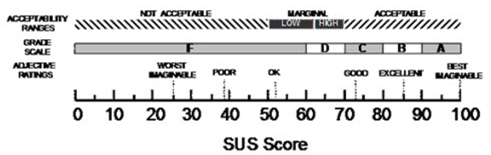
\includegraphics [width = 13cm, height= 4.5cm]{gambar/sus}}
	\caption{SUS \textit{Score} \citep{bangor2009determining}}
	\label{sus}
\end{figure}

%-----------------------------------------------------------------------------%

% Baris ini digunakan untuk membantu dalam melakukan sitasi
% Karena diapit dengan comment, maka baris ini akan diabaikan
% oleh compiler LaTeX.

\fancyhf{} 
\fancyfoot[R]{\thepage}

\begin{comment}
\bibliography{daftar-pustaka}
\end{comment}